%----------------------------------------------------%
%       ANÁLISIS DE LAS TÉCNOLOGÍAS PROPUESTAS       %
%----------------------------------------------------%

\pagestyle{fancy}

\chapter{Análisis de las tecnologías propuestas}
\label{analisis_tecnologias}

\section{Apache Cassandra}

Apache Cassandra es una base de datos NoSQL distribuida desarrollada por DataStax bajo la licencia de Apache que permite operar con grandes volúmenes de datos del tipo clave/valor. Las principales ventajas que ofrece respecto a bases de datos homologas son una mayor escalabilidad lineal y disponibilidad total de los datos. Para lograr dichas ventajas se basa en una serie de nodos homogéneos que se comunican entre ellos mediante un protocolo P2P de replicación asincrónica, lo cual permite realizar operaciones de baja latencia para todos los clientes sin necesidad de un servidor maestro.\\

En 2012, investigadores de la Universidad de Toronto que estudian los sistemas NoSQL concluyeron que "En términos de escalabilidad, hay un claro ganador a través de nuestros experimentos. Cassandra logra el más alto rendimiento para el número máximo de nodos en todos los experimentos"[].\\

Actualmente está siendo utilizada por muchas de las aplicaciones en negocios modernos, siendo la base de datos elegida por un cuarto de las empresas de la Fortune 100[]. Claro ejemplo de ello son empresas mundialmente conocidas como Apple, Facebook o NetFlix, los cuales utilizan Cassandra como parte de su entramado tecnológico desde hace ya unos años. Cabe destacar que su uso no se limita al mundo empresarial. Muestra de ello es la acogida que ha tenido en el ámbito de la investigación, formando parte en experimentos punteros a nivel mundial como algunos de los realizados en el CERN[].\\

Es indispensable tener en cuenta que no se trata de una base de datos de propósito general, por lo que, es de vital importancia conocer cuando se va a poder exprimir su potencial al máximo y cuando no.\\

Será \textbf{recomendable} utilizar Cassandra si:

\begin{itemize}
	\item se desea que la configuración, mantenimiento y el código sea sencillo.
	\item se necesitan velocidades muy altas en lecturas y escrituras aleatorias.
	\item no se necesitan múltiples índices secundarios
	\item existe alta flexibilidad en la estructura de los datos
	\item se busca una escalabilidad masiva
	\item se busca alta disponibilidad
\end{itemize}

\textbf{No} será \textbf{recomendable} utilizar Cassandra si:

\begin{itemize}
	\item se manejan datos relacionales
	\item hay transacciones de por medio
	\item se requiere autorización para acceder a datos
	\item se necesita latencia baja
\end{itemize}

\subsection{Funcionamiento}

Debido al modelo distribuido sobre el cual esta desarrollado, el primer paso para comprender el funcionamiento de Apache Cassandra es familiarizarse con los conceptos básicos de los sistemas distribuidos y entender como se aplican sobre esta tecnología en concreto.\\

El Teorema de Brewer[], también conocido como Teorema CAP , enuncia que es imposible para un sistema de cómputo distribuido garantizar simultáneamente las tres propiedades que se presentan a continuación, solo pudiendo cumplir dos de ellas al mismo tiempo, y acabar cumpliendo el restante tarde o temprano.\\

\begin{itemize}
	\item \textbf{Consistencia}(Consistency): Todos los nodos ven la misma información al mismo tiempo.
	\item \textbf{Disponibilidad}(Availability): La garantía de que cada petición a un nodo reciba una confirmación de si ha sido o no resuelta satisfactoriamente.
	\item \textbf{Tolerancia al Particionado}(Partition Tolerance): El sistema sigue funcionando a pesar de que haya sido partido por fallo de red.
\end{itemize}

Para una base de datos distribuida que promete la disponibilidad completa, como lo es Cassandra, el Teorema de Brewer implica la imposibilidad de garantizar la consistencia total en el sistema y la necesidad de esperar un tiempo indeterminado para que las réplicas de un registro modificado se actualicen correctamente.\\

No obstante, existen formas de minimizar el tiempo necesario para alcanzar un estado consistente. La primera, es proveer la infraestructura de medios físicos necesarios para acelerar el intercambio de datos entre los nodos y evitar que la red se congestione en el proceso. La segunda, trata sobre la posibilidad que Cassandra ofrece de elegir el nivel de consistencia() con el que se ejecuta cada consulta.\\

Otra de las características heredada de bebido a su naturaleza distribuida es el uso de un protocolo Gossip para lograr que todo el entramado funcione de manera coordinada. Mediante paso de mensajes periódicamente se da a conocer el estado de un nodo al resto de sus vecinos, posibilitando de esa manera, que cada nodo pueda mantener actualizadas sus réplicas.\\

Pasando a las caracteristicas propias de Cassandra...

%En una base de datos relacional como MySQL, las tablas son diseñadas con el objetivo de minimizar la redundancia de los datos que, a la poste, se almacenarán en ella, siguiendo para lograr dicho objetivo un proceso de normalización[] estandarizado desde hace ya décadas. Al operar con Cassandra, en cambio, las tablas se construyen buscando una respuesta rápida a las consultas que se realizan sobre ella, hecho que afecta de forma directa

tablas orientadas a consultas

patition key etc

Ilustración 5. Estructura de Cassandra

Apache Cassandra posibilita almacenar réplicas de un mismo registro en diferentes nodos del clúster. Al crear un keyspace, homólogo de una base de datos en MySQL, permite especificar el factor de replicado, número entero que representa la cantidad de copias que se desean almacenar en la infraestructura. Cada nodo posee una réplica para un cierto rango de datos y si uno de ellos falla, otro que posea dicha réplica puede responder a la petición sin tener que interrumpir el servicio.\\ 

Otro de los atributos que se debe especificar a la hora de crear un keyspace es el denominado Replica Placemente Startegy, atributo que indica cómo se han de repartir los registros replicados por el anillo. Ofrece la posibilidad de 

implicaciones que tiene todo ello

\begin{figure}[h]
	\centering
	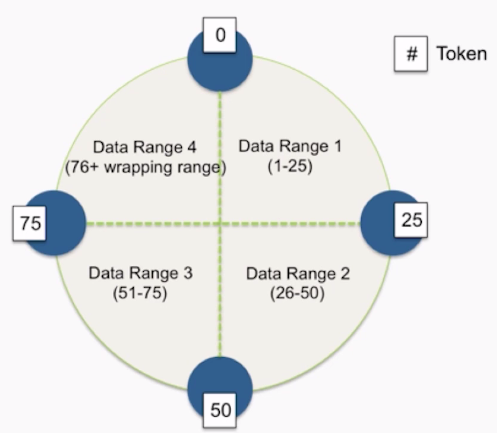
\includegraphics[width=0.5\textwidth]{Ilustraciones/cassandra_token.png}
	\caption{Particionamiento en Cassandra}
	\label{fig:cassandra_token}
\end{figure}




%En cuanto a la estructura se refiere, un keyspace es un espacio de nombres para un conjunto de ColumFamily. Por lo general se utiliza uno por aplicación y es considerado el equivalente a una base de datos del modelo relacional. El ColumFamily, a su vez, es capaz de almacenar diferentes columnas, siendo el homologo de una tabla del modelo relacional. Para finalizar, una columna seria una estructura compuesta por clave, valor y timestamp.

%Cabe mencionar que el almacenamiento de las columnas en a base de datos no es aleatoria. Cassandra almacena los datos dependiendo del primer atributo especificado en la clausula primary_key a la hora de crear el ColumFamily, guardando en el mismo nodo las columnas que comparten el valor de dicho atributo. Por ejemplo, si se especificarán las dos siguientes claves primarias:

%En ambos casos la clave primaria vendría a ser la misma, la combinación de los tres atributos que aparecen entre paréntesis. No obstante, Cassandra no almacenaría los datos de igual forma en ambos casos. En el primero, los datos con un mismo username serían almacenados en el mismo nodo o en nodos vecinos a este, mientras que en la segundo, los datos almacenados siguiendo ese criterio de proximidad serían los que coincidiesen en username e interaction_date.

\subsection{Cassandra Query Lenguage (CQL)}

permite conectarse al cualquier nodo del cluter (homogeneidad)

Apache Cassandra posee su propio lenguaje de consultas, el denominado Cassandra Query Lenguage (CQL). Su sintaxis guarda una gran similitud con la de SQL, lo cual facilita, de forma notoria, el salto que supone pasar de trabajar con bases de datos relacionales a distribuidos.\\

Aún siendo sintácticamente  tan parecido a SQL, presenta ciertas restricciones debido a que es un lenguaje de consultas de una base de datos distribuida. Por ejemplo, no ofrece la posibilidad de realizar operaciones como JOIN y es totalmente necesario especificar todas los atributos que componen la clave primaria a la hora de realizar cualquier consulta de filtrado o de actualización en la tabla. La única operación que no cumple esta restricción es un select que contenga la clausula where, ya que, al definir la clave primaria Cassandra indexa de forma automática todos sus componente, posibilitando más tarde  hacer uso de ellos en este caso concreto.

Otra de las peculiaridades que presenta CQL es el hecho de ofrecer dos modos distintos de realizar un update. El primero de todos es el mencionado en el párrafo anterior. El segundo posibilita actualizar una columna realizando un insert repitiendo el valor de las claves primarias de una columna ya existente en la base de datos. Esta segunda forma es cómoda a la par de peligrosa porque Cassandra no notifica si una clave primaria ya existe en la base de datos o no, pudiendo un insert desencadenar en un update no deseado.  


\section{Apache Spark}

Apache Spark[9] es un proyecto open source de computación en clúster. Desde el principio fue diseñado para poder ejecutar algoritmos iterativos en memoria sin la necesidad de almacenar en disco los resultados intermedios generados durante el proceso. Esta peculiaridad permite que los procesamientos llevados a cabo con Spark puedan llegar a ser, en algunos casos concretos, 100 veces más rápidos que los de MapReduce[10].\\

A mediados de 2014, coincidiendo con el lanzamiento de la primera versión, alcanzó la cifra de 465 colaboradores, convirtiéndolo en el proyecto más activo entre los relacionados con el Big Data dentro de la Apache Software Fundation.\\

Apache Spark está compuesto por múltiples y variados componentes que pueden ser utilizados de forma conjunta.\\

\begin{figure}[h]
	\centering
	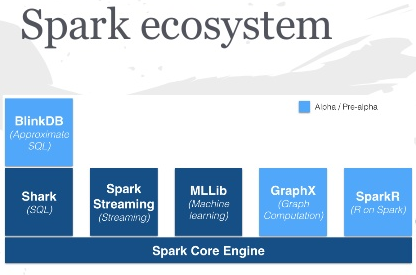
\includegraphics[width=0.5\textwidth]{Ilustraciones/spark_ecosystem.png}
	\caption{Ecosistema Spark}
	\label{fig:ipanel}
\end{figure}

La base del proyecto es el denominado Spark Core. Proporciona envío distribuido de tareas, planificación y funciones básicas de entrada salida. La abstracción fundamental de programación se llama Resilient Distributed Datasets (RDD)[11], una colección lógica de datos particionados a través de las máquinas que se expone mediante una API integrada en lenguajes como Java, Python y Scala.\\

\subsection{Funcionamiento}

Para el funcionamiento de Spark, es condición sine qua non que los nodos de la infraestructura tengan acceso a la totalidad de los datos que se desea tratar. Ello implica que para procesar un fichero de 50GB, cada nodo tendría que poseer una copia del mismo almacenado en su disco. Esta praxis es inviable, ya que más allá de los problemas de consistencia que generaría, para nada es eficiente ocupar la memoria de todos los nodos con información redundante y procesar el fichero entero cuando en realidad se va a hacer uso de una pequeña porción de dichos datos en cada ejecución.\\

Las bases de datos distribuidas como Cassandra solventan los problemas anteriormente mencionados. Se encargan de distribuir los datos entre diferentes nodos del clúster, ofrecen la posibilidad de acceder a ellos desde cualquier punto y mantienen la consistencia de los mismos a cambio de sufrir una pequeña latencia en el caso de requerir información almacenada en otro nodo de la infraestructura.\\ 

Al ejecutar una aplicación que opera con Spark, un componente denominado driver es lanzado. Debido a la necesidad de obtener recursos (CPU y memoria) para llevar a cabo la computación que se le ha encomendado, se comunica con un nodo del clúster que, mediante especificación previa, adopta el rol de maestro. Éste pregunta a todos los nodos que conforman la infraestructura sobre la cantidad de recursos disponibles que poseen y así asignarles los executors correspondiente. Las máquinas que alojen al menos un executor pasan a denominarse worker y a partir de este momento, cada executor podrá comunicarse directamente con el Driver para poder recibir las tareas que éste le envíe.\\

Un executor es una unidad de trabajo que se encarga de computar las tareas que le encomienda el driver. El número de executors que puede albergar cada worker está directamente relacionado con el número de procesadores que este posee. De la misma forma, es posible repartir la memoria RAM que dispone el nodo worker entre varios executors. Spark permite modificar ambos parámetros programáticamente permitiendo así poder amoldarse a las particularidades de cada ejecución.\\

Para transferir el código del programa, residente en la máquina del driver, éste adopta  el rol de servidor e intenta enviar dicho código a los workers. Si el fichero JAR que contiene el código ha sido recibido correctamente por sus destinatarios, estos responden mediante un ACK y en caso contrario, se vuelve a intentar el envío un número determinado de veces. Una vez llegado al máximo de reintentos, el worker que no haya enviado el ACK es considerado como caído, quedando los executors que albergaba fuera del posterior reparto de tareas.\\

\begin{figure}[h]
	\centering
	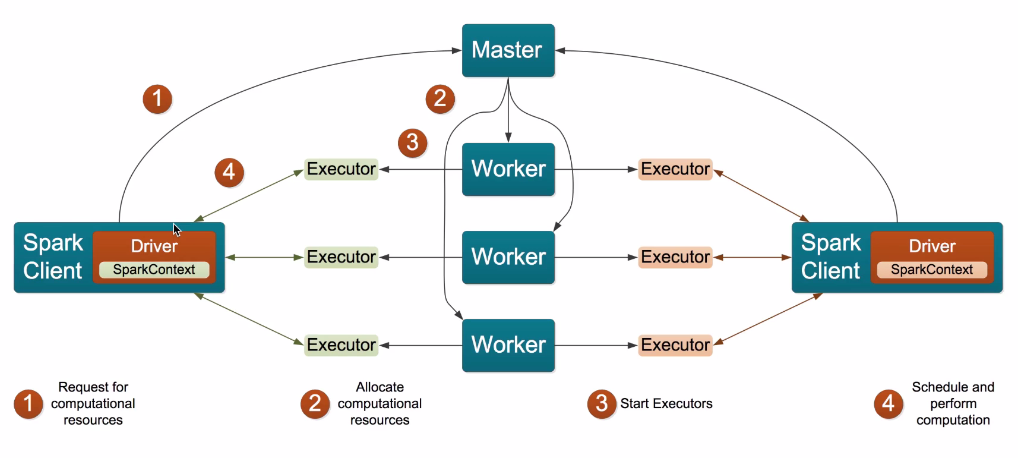
\includegraphics[width=1\textwidth]{Ilustraciones/spark_architecture.png}
	\caption{Arquitectura Spark}
	\label{fig:spark_architecture}
\end{figure}

A la hora de realizar operaciones en Spark, el objeto estrella es el denominado Resilient Distributed Datasets (RDD)[11]. Se trata de una abstracción que mediante diferentes APIs disponibles para Java, Scala y Python permite manipular datos distribuidos por los diferentes nodos del clúster como si estuvieran almacenados de forma local. Este objeto es inmutable, lo cual implica que una vez creado no se le pueden añadir nuevos elementos o eliminar los existentes, solo aplicar transformaciones y acciones sobre el.\\

Las operaciones que se pueden realizar sobre las RDD se agrupan, tal y como se ha adelantado antes, por transformaciones y acciones. Las primeras transforman un RDD en otro según el criterio indicado y las segundas realizan modificaciones sobre los datos almacenados en dichas RDD. Cabe destacar que las transformaciones en Spark son operaciones "lazy", lo cual implica que en realidad cada nodo memoriza la secuencia de transformaciones que ha de realizar y los procesa cuando una acción es ejecutada.\\

Una vez terminada la primera fase en la que los executor son creados y enlazados con el driver, éste último empieza a analizar la estructura del código y genera un grafo DAG (Directed Acyclic Graph) con las operaciones que se realizan sobre la RDD. Partiendo de ese grafo genera un job por cada operación de tipo acción que encuentra y dentro de cada job separa la ejecución en diferentes stages según las dependencias que existan entre operaciones. Por último, cada stage es dividido por defecto en unidades de 64MB y a cada unidad resultante se denomina task, el cual es enviado a un executor para ser procesado. El tamaño de cada task puede ser modificado programáticamente, pudiendo de esa forma manipular el número de task que un executor deba ejecutar.\\

\begin{figure}[h]
	\centering
	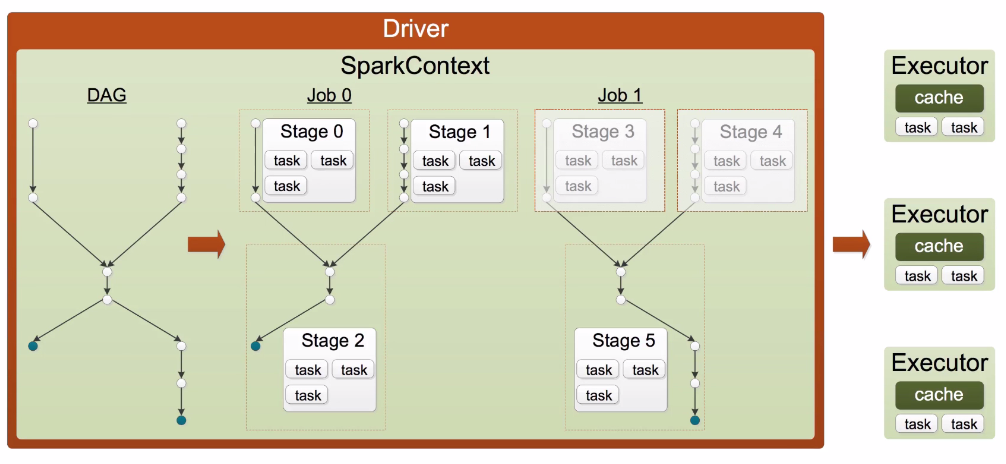
\includegraphics[width=1\textwidth]{Ilustraciones/spark_task_creation.png}
	\caption{Arquitectura Spark}
	\label{fig:spark_task_creation}
\end{figure}

El driver, una vez habiendo recibido los resultados de todas los task que ha repartido, enviará un mensaje a los executors indicando que el procesamiento ha sido finalizado y calculará el resultado final ofreciendo la posibilidad de, por ejemplo, almacenarlo en una base de datos distribuida como Cassandra.\\






